\papersubsection{Exception handling}


%This section evaluates the performance of handling an exception from the host OS or hardware,
%including installing an exception handler,
%interrupting a running thread
%with \palcall{ThreadInterrupt} (raising an \code{INTERRUPT} exception in the target thread),
%and catching a hardware protection fault
%(writing to a read-only address).


Exception handling on \thehostabi{}
includes installing upcall functions as handlers to exceptions,
and delivery of exceptions to the installed handler.
Handler installation
is relatively fast on almost every PAL implementation.
For the Linux PAL and \sgx{} PAL,
handler installation
is at least 6\x{} faster than calling \syscall{sigaction} on native Linux (Figure~\ref{fig:eval:pal:sig-latency}),
because the \hostapi{} only has to update a function pointer in the process.
However, exception delivery
tends to be a much more expensive operation,
due to implementing various corner cases
upon restrictions
of host OSes or hardware.
%and a user-space
%implementation tends to be less efficient
%than the host OS.

%Both the Linux PAL and \sgx{} PAL implement an elaborate exception delivery scheme
%which gracefully handles
%corner cases
%of hardware or OS-triggered exceptions.
%One corner case
%that the PALs handle
%is an internal exception,
%which happens during either a \hostapi{} or the host exception handler in the PAL.
%The PALs
%detect these internal exceptions
%and roll back the stack
%to the latest guest frame.
%As shown in Figure~\ref{fig:eval:pal:sig-latency},
%delivering a memory fault on the Linux PAL
%is up to 273\%
%more expensive than delivering a \code{SIGSEGV} signal
%to a native Linux process.



Both the Linux PAL and \sgx{} PAL implement
an elaborate exception delivery scheme
to handle various corner cases where exception can happen.
First, \thehostabi{}
defines several types of exceptions,
which are all delivered through a unified interface.
The deliverable exceptions
include hardware exceptions such as memory faults,
arithmetic errors (divide-by-zero), and illegal instructions,
and OS-triggered exceptions
such as system calls forbidden by the \seccomp{} filter.
On the Linux PAL,
most exceptions are delivered as signals.
However, on the \sgx{} PAL,
hardware exceptions are delivered directly into enclaves,
with the interrupted register contexts dumped
into a designated area called SSA (state save area).
Moreover, exceptions can happen
either in the guests (i.e., applications and \liboses{})
or inside the PAL code or a PAL exception handler.
To gracefully handle these corner cases,
both the Linux PAL and \sgx{} PAL examines the saved register values to determine the reasons and code addresses
that raise the exceptions.



Figure~\ref{fig:eval:pal:sig-latency} shows the overheads
on exception delivery
on the two PAL implementations,
based on two corner cases:
(1) interrupting the current thread (similar to sending \code{SIGUSR1});
(2) delivering a memory protection fault
from the application.
For thread interruption,
because the exception happen in the middle of a \hostapi{},
the overhead is only 37\%
on the Linux PAL.
However,
the latency of the Linux PAL
to deliver a memory fault from the application
is up to 273\% slower
than the similar operation on native Linux;
the primary reason of
the significant slowdown
is to deliver the exception information
from the host OS,
including the faulting address
and interrupted register contexts.


%If the application triggers
%a memory protection fault, the Linux PAL receives an signal in its own handler
%and delivers the exception with
%a copy of the interrupted context to the guest handler.
%After the guest handler returns,
%the Linux PAL applies the changes on the interrupted context
%and restores the execution.
%The overall overhead for delivering a memory fault
%on the Linux PAL
%is up to 273\%.




%Without virtualizing interrupt handlers,
%a hardware exception
%on the Linux PAL are delivered into the host Linux kernel
%and then sent to the process as a signal.
%The host Linux kernel
%also delivers
%OS-trigger exceptions,
%such as interruption from another thread
%and blocked system calls,
%as different signals (e.g., \code{SIGUSR1} and \code{SIGSYS}) to the process.
%Processing these
%host signals involves several expensive operations,
%including
%checking the ranges of interrupted instructions
%and passing the register files
%to the guest exception handlers.
%For delivering a memory fault,
%the overheads add up to \roughly{}273\%.
%%Similar overheads are observed on the delivery of other exceptions.
%%Delivering other exceptions can expect
%%a similar overhead.


For the \sgx{} PAL,
exception delivery is dominated
by enclave exits.
Although the \sgx{} PAL does not trust the untrusted OS to deliver exceptions,
\sgx{} forces
enclave execution
to stop and exit to the untrusted OS
at exception,
causing significant overheads
on exception handling.
Moreover, to handle a hardware exception such as memory fault or illegal instruction,
the \sgx{} PAL has to
effectively exit an enclave twice,
one for handing the exception and
the other for freeing
the limited SSA (state save area).
%As a result,
On the \sgx{} PAL,
the overhead on delivering a memory fault
is nearly twice as the overhead on thread interruption. 



\begin{figure*}[t!]
\centering
\footnotesize
\resizebox{\textwidth}{!}{%
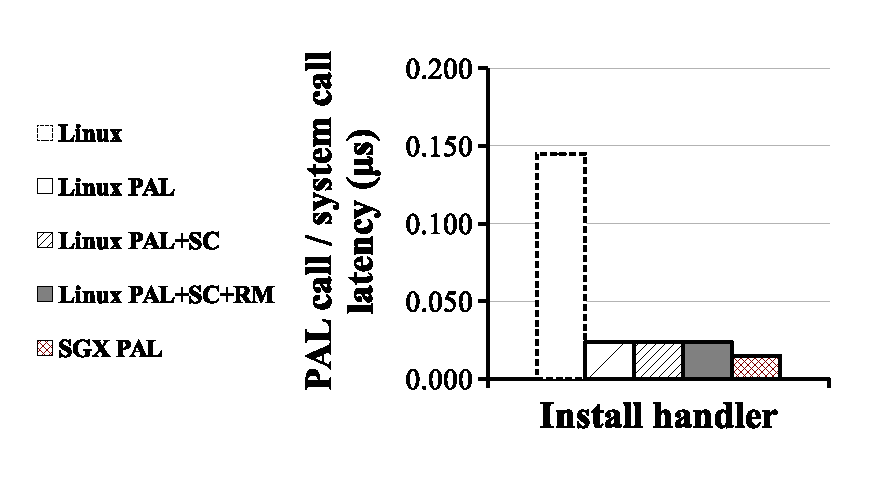
\includegraphics[height=10em]{sig-install-latency}
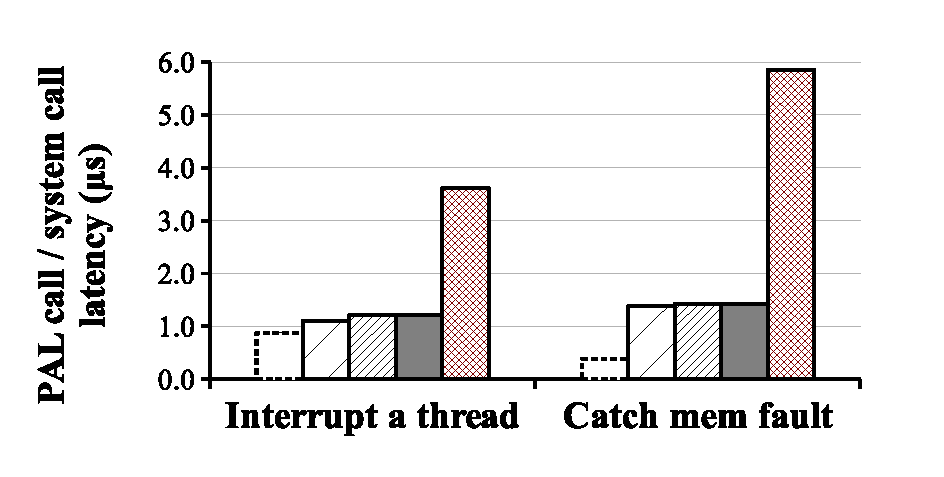
\includegraphics[height=10em]{sig-catch-latency}
}
\caption{Latency of (a) installing an exception handler; (b)
interrupting a running thread with signals (on Linux) or \palcall{ThreadInterrupt} on the PALs; (c) catching a memory protection fault. Lower is better. The comparison is between (1) signals on Linux; (2) the Linux PAL, with and without a \seccomp{} filter ({\bf +SC}) and reference monitor ({\bf +RM}); (3) the \sgx{} PAL.}
\label{fig:eval:pal:sig-latency}
\end{figure*}


%Figure~\ref{fig:eval:pal:sig-latency} (a)
%shows the latency of installing an exception handler in either the Linux or \sgx{} PAL, compared with
%\syscall{sigaction} in a Linux process.
%The result
%shows that regardless the PAL is running in a regular \picoproc{} or an enclave,
%installing an exception handling
%in the PAL
%is much lower than install a signal handler
%on Linux,
%because the \hostapi{} does not have to take any system call or enclave exits.


%Figure~\ref{fig:eval:pal:sig-latency}
%measures the latency of delivering an interrupt and a memory protection exception
%to a thread in the process.



%Figure~\ref{fig:eval:pal:sig-latency} (b)
%shows the latency of interrupting a running thread
%and raising an exception
%in the target thread, compared with delivering a \code{SIGUSR1} signal in a Linux process.
%Thread interruption on the Linux PAL
%is slightly slower than
%delivering a \code{SIGUSR1} signal,
%by \roughly{}25\% without \seccomp{} filter and reference monitor, or \roughly{}32\% with \seccomp{} filter and reference monitor.
%On the \sgx{} PAL,
%the latency of thread interrupt
%is much higher, due to the cost of extra thread exits.
%Interrupting a thread running on the \sgx{} PAL
%is \roughly{}3.1\x{} shower than delivering a \code{SIGUSR1} signal in a Linux process.



%Figure~\ref{fig:eval:pal:sig-latency} (b)
%shows the latency of catching a memory protection fault,
%compared with handling
%a \code{SIGSEGV} signal in a Linux process.
%On the Linux, handling a hardware fault is \roughly{}2.6\x{} slower than handling a \code{SIGSEGV} signal on Linux;
%such an overhead
%is primarily caused by delivering
%the exception information to the guest, including the faulting register contexts.
%Figure~\ref{fig:eval:pal:sig-latency} (b)
%also shows that catching a hardware fault inside an enclave
%is even more expensive
%than thread interruption, by nearly 60\%.
%The reason of such a dramatic difference is that
%interrupting a thread only causes the interrupt thread to exit and enter the enclave once,
%whereas handling a hardware fault
%requires the faulting thread to exit and enter the enclave twice,
%in order to reset the in-enclave buffer
%for preserving the faulting contexts.


